\documentclass[10pt,a4paper]{article}
\usepackage[utf8]{inputenc}
\usepackage{amsmath}
\usepackage{amsfonts}
\usepackage{amssymb}
\usepackage{graphicx} 
\usepackage{subfigure} 
\author{Oscar Daniel Juárez Cruz}
\title{Práctica 1}
\begin{document}
\maketitle

\section{Introducción}
En un sistema multiprogramado o de tiempo compartido, un proceso es la
imagen en memoria de un programa, junto con la información relacionada con
el estado de su ejecución.
Un programa es una entidad pasiva, una lista de instrucciones; un proceso
es una entidad activa, que –empleando al programa– define la actuación que
tendrá el sistema. \\\\
Un proceso, a lo largo de su vida, alterna entre diferentes estados de ejecución.
Éstos son: \\
\begin{itemize}
	\item Nuevo: Se solicitó al sistema operativo la creación de un proceso, y sus recursos y estructuras están siendo creadas.
	\item Listo: Está listo para iniciar o continuar su ejecución pero el sistema no le ha asignado un procesador.
	\item En ejecución: El proceso está siendo ejecutado en este momento. Sus instrucciones están siendo procesadas en algún procesador.
	\item Bloqueado: En espera de algún evento para poder continuar su ejecución (aun si hubiera un procesador disponible, no podría avanzar).
	\item Zombie: El proceso ha finalizado su ejecución, pero el sistema operativo debe realizar ciertas operaciones de limpieza para poder eliminarlo de la lista.
	\item Finalizado: El proceso terminó de ejecutarse; sus estructuras están a la espera de ser limpiadas por el sistema operativo.
\end{itemize}
\newpage

\section{Desarrollo}

\begin{flushleft}
La práctica consiste en crear un árbol de procesos que cree primero el hijo izquierdo y derecho y posteriormente la rama izquierda crear 'n + 1' hijos, y la rama derecha constante de 3 hijos
\end{flushleft}

A continuación observamos el diagrama de flujo del programa.

\begin{center}
	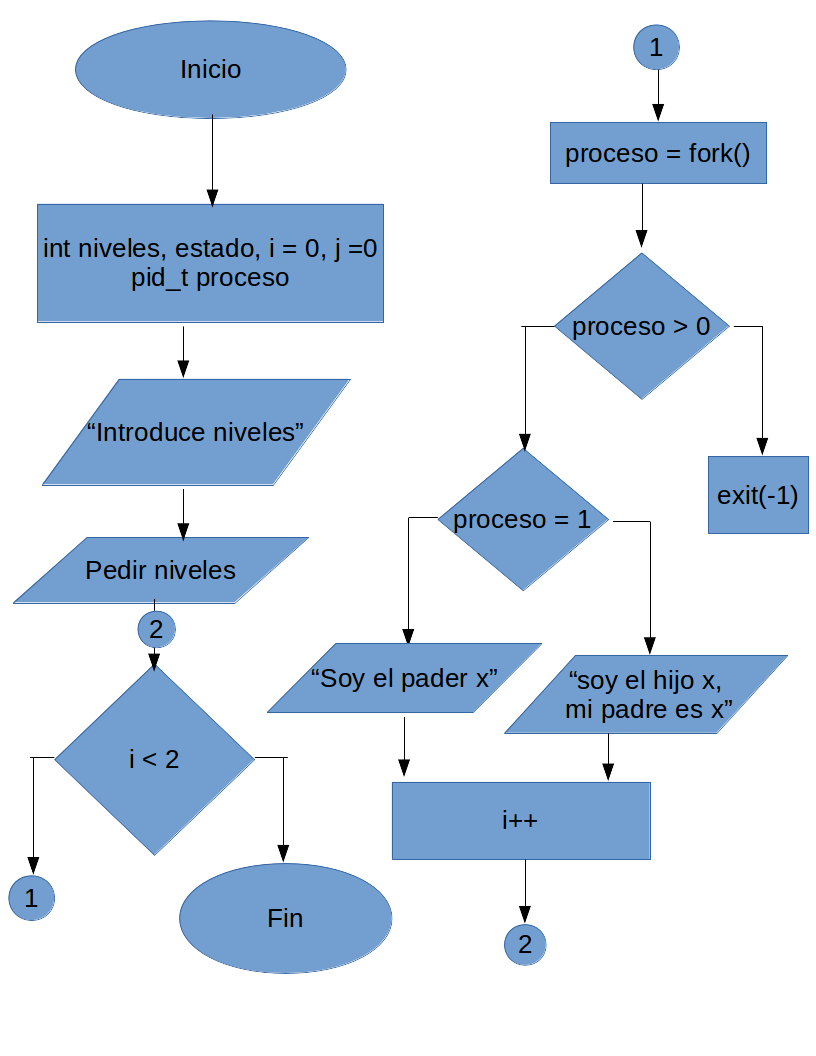
\includegraphics[scale=0.3]{diagrama.png} 
\end{center}

En el diagrama podemos observar que inicialmente se crean los dos hijos: izquierdo y derecho. Mediante una función recursiva se crean los hijos de los hijos de manera recursiva.\\\\

A continuación observamos la función:

\begin{center}
	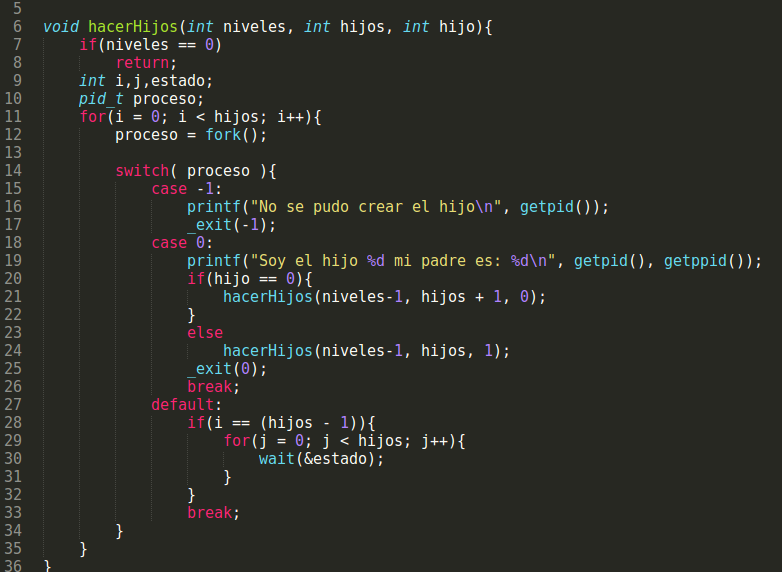
\includegraphics[scale=0.35]{codigo.png} 
\end{center}

\begin{flushleft}
\textbf{Función: hacerHijos()} 
\end{flushleft}

\begin{flushleft}
Parámetros: int niveles, int hijos, int hijo\\
\end{flushleft}
\begin{flushleft}
Especificación: \\
niveles: el número de niveles que quieres crear \\
hijos: el número de hijos que quieres crear \\
hijo: 0 si se trata del hijo izquierdo o 1 si se trata del hijo derecho \\
\end{flushleft}

\begin{flushleft}
Descripción:\\
La función crea el número de hijos que requiere con el padre a través de un contador.\\
Hay un contador principal para poder crear los procesos que se requieren y dentro de las funciones de los hijos están la recursividad en la función para poder volver a llamarla una vez que se creen los hijos. \\
Simultáneamente se van imprimiendo los pid's de los procesos.
\end{flushleft}

\begin{flushleft}
Return: \\
La función no regresa ningún valor.
\end{flushleft}

\subsection{Ejemplo}

\begin{flushleft}
En el siguiente ejemplo observaremos el programa corriendo con el valor de 3 niveles. \\
Utilizamos un árbol para vaciar el output y observar cómo se crea la estructura.
\end{flushleft}

\begin{center}
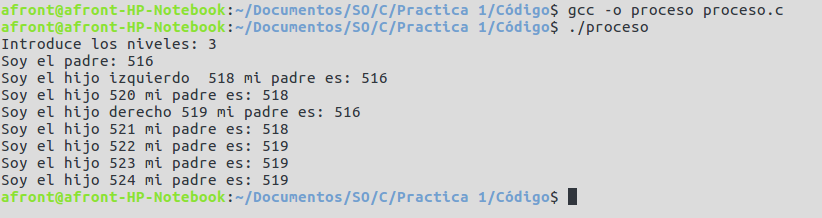
\includegraphics[scale=0.3]{example.png} \\
Output del programa
\end{center}

\begin{flushleft}
Construyendo el árbol...
\end{flushleft}

\begin{center}
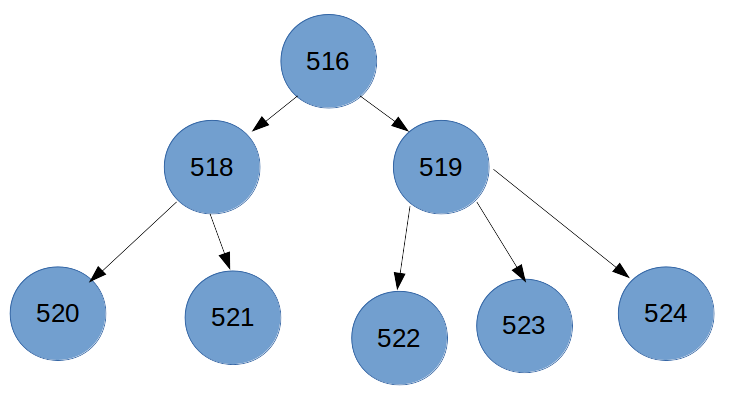
\includegraphics[scale=0.3]{arbol.png} \\
Árbol con la salida
\end{center}

\section{Conclusiones}

\begin{flushleft}
La desición de qué proceso se imprime primero sale de nuestras capacidades puesto que, el planificador es quien decide qué prioridad asignarlos por lo que no nos es posible administrar la forma en la que se imprimen los procesos hijos y padres.
\end{flushleft}

\begin{flushleft}
A lo largo de la práctica existieron algunos problemas de desarrollo sobre todo para poder manera la manera en que los procesos se tienen que volver a ocupar para crear a sus hijos pero utilizando correctamente la función de \textit{wait} y la funcion de \textit{exit} logramos que estos se hicieran de manera recursiva y así se pudiesen crear todos.
\end{flushleft}

\end{document}